\documentclass[../Main.tex]{subfiles}

\begin{document}
\section{Basics of Dual Spaces}
\begin{definition}{Dual space}
    Let $V$ be a vector space over a field $\F$. The \underline{dual space} of $V$ is:
    \begin{equation*}
        V^* = \L(V, \F)
    \end{equation*}
    and an element $\theta \in V^*$ is sometimes known as a \underline{linear functional} on $V$.
\end{definition}
Let $B$ be a basis for $V$ and $b \in V$. Then the dual of this basis vector is:
\begin{equation*}
    b^* : \sum_{c \in B} \lambda_c c \mapsto \lambda_b
\end{equation*}
and the restriction $b^*|_B$ is just $\delta_{b, c}$. We then define the dual basis $B^* = \subsetselect{b^*}{b \in B}$.
\begin{proposition}
    For $V, B, B^*$ as defined above, $B^*$ is linearly independent.

    If $V$ is finite-dimensional then $B^*$ is a basis for $V^*$.
    \label{propDualBasis}
\end{proposition}
\begin{proof}
    For linear independence find a zero linear combination and by applying this to each basis vector show that the coefficients must in fact be zero.

    Then argue by dimensions for the second part.
\end{proof}
\begin{corollary}
    For a finite-dimensional vector space $V$, $V \isom V^*$.
    \label{corDualSpaceIsom}
\end{corollary}
\begin{proof}
    Extend an isomorphism of bases.
\end{proof}
\begin{definition}{Annihilator}
    For $V$ a vector space over $\F$, $S \subseteq V$, the \underline{annihilator} of $S$ is:
    \begin{equation*}
        S^0 = \subsetselect{\theta \in V^*}{\theta(s) = \zv_V~\forall s \in S}
    \end{equation*}
\end{definition}
\begin{propositions}{
        Let $V$ be a finite-dimensional vector space over $\F$ with subsets $S$ and $T$.
        \label{propsAnnihProps}
    }
    \item $S^0 \leq V^*$; \label{propAnnihSubspace}
    \item if $S \subseteq T$ then $T^0 \leq S$; \label{propAnnihSubsetReverse}
    \item $S^0 = \spn{S^0}$; \label{propAnnihIsSpan}
    \item $V^0 = \{\zv_{V^*}\}$ and $\{\zv_V\}^0 = V^*$ \label{propAnnihOfZero}
\end{propositions}
\begin{proof}
    For 1, apply the subspace test. For 2, argue by the definitions. In 3, 2 gives us one inequality so we have to show the other. Do this by linear combinations.
    
    Finally, 4 is trivial.
\end{proof}
\begin{proposition}
    For $V$ finite dimensional, and $U \leq V$,
    \begin{equation*}
        \dim(V) = \dim(U) + \dim(U^0)
    \end{equation*}
    \label{propDimAnnih}
\end{proposition}
\begin{proof}
    Extend a basis of $U$ to a basis of $V$, and show that the dual of the added basis vectors are exactly the basis of $U^0$.
\end{proof}
\begin{propositions}{
        Let $V$ be a vector space over $\F$. Let $U, W \subseteq V$.
        \label{propsAnnihSums}
    }
    \item $U^0 \cap W^0 = (U + W)^0$;
    \item $U^0 + W^0 \leq (U \cap W)^0$;
    \item If $V$ is finite-dimensional then we have equality in 2.
\end{propositions}
\begin{proof}
    For 1, show that $LHS \subseteq RHS$ and vice versa.

    For 2, use \thmref{propAnnihSubsetReverse}. In the finite-dimensional case, use \thmref{propDimAnnih} and \thmref{corSumIntersection}.
\end{proof}
\section{Dual Linear Maps}
\begin{definition}{Dual map}
    Let $\alpha \in L(V, W)$. Then the \underline{dual map} of $\alpha$ is given by:
    \begin{align*}
        \alpha^* : W^* &\mapsto V^*\\
        \theta &\mapsto \theta \circ \alpha
    \end{align*}
\end{definition}
Figure~\ref{figDLMDiagram} aids this definition.
\begin{figure}
    \centering
    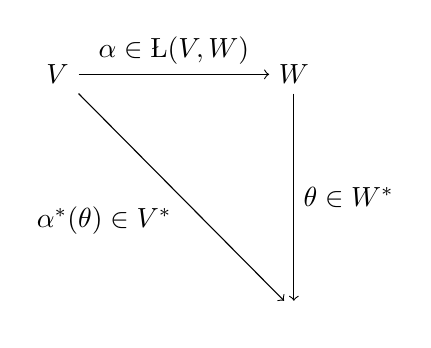
\begin{tikzpicture}[scale=3]
        \node (V) at (0, 0) {$V$};
        \node (W) at (1, 0) {$W$};
        \node (F) at (1, -1) {$\F$};

        \draw[->] (V.east) -- (W.west)
            node[pos=0.5, anchor=south] {$\alpha \in \L(V, W)$};
        \draw[->] (W.south) -- (F.north)
            node[pos=0.5, anchor=west] {$\theta \in W^*$};
        \draw[->] (V.south east) -- (F.north west)
            node[pos=0.5, anchor=north east] {$\alpha^*(\theta) \in V^*$};

    \end{tikzpicture}
    \caption{Diagram of Dual Linear Maps}
    \label{figDLMDiagram}
\end{figure}
\begin{propositions}{
        Let $\alpha, \beta \in L(V, W)$ and $\gamma \in L(U, V), \lambda \in \F$. THen:
        \label{propsDLMProps}
    }
    \item $\alpha^*$ is linear;
    \item $(\alpha + \lambda \beta)^* = \alpha^* + \lambda \beta^*$ (starring is a linear operation);
    \item $(\alpha \circ \gamma)^* = \gamma^* \circ \alpha^*$;
    \item $(\Id_V)^* = \Id_{V^*}$ (starring preserves identity);
    \item If $\beta$ is an isomorphism then so is $\beta^*$ with inverse:
        \begin{equation*}
            (\beta^*)^{-1} = (\beta^{-1})^*
        \end{equation*}
\end{propositions}
\begin{proof}
    For all of these, just argue by the definitions (and use previous parts of the proposition).
\end{proof}
\begin{proposition}[Matrix of a dual linear map]
    Let $V, W$ be finite-dimensional vector spaces with bases $B$ and $C$, respectively. For $\alpha \in \L(V, W)$,
    \begin{equation*}
        [\alpha^*]^{C^*}_{B^*} = \left([\alpha]^B_C\right)^T
    \end{equation*}
    \label{propDLMMatrix}
\end{proposition}
\begin{proof}
    Prove directly by finding the elements of the matrix of $\alpha^*$.
\end{proof}
\begin{corollary}
    Under the same assumptions as \thmref{propDLMMatrix}, $\rk(\alpha^*) = \rk(\alpha)$.
    \label{corDLMSameRank}
\end{corollary}
\begin{propositions}{
        Let $V, W$ be vector spaces over a field $\F$. For $\alpha\in\L(V, W)$,
        \label{propDLMKernel}
    }
    \item $\ker(\alpha^*) = \im(\alpha)^0$; \label{propDualKernel}
    \item $\im(\alpha^*) \leq \ker(\alpha)^0$; \label{propDualImage}
    \item If $V$ and $W$ are finite-dimensional then we have equality in 2. \label{propDualImageFinite}
\end{propositions}
\begin{proof}
    1 is simple by proving that both sides fit inside the other. Similar for the first direction of 2.

    For 3, use \thmref{corDLMSameRank} and argue by dimension.
\end{proof}
\section{The Double Dual}
\begin{theorem}[Natural Isomorphism]
    Let $V$ be a vector space over $\F$. Then there exists a linear map given by:
    \begin{align*}
        E : V &\mapsto V^{**}\\
        v &\mapsto v^{**}
    \end{align*}
    where $v^{**}(\theta) = \theta(v)$ for $\theta \in V^*$.
    \label{thmNaturalIsomorphism}
\end{theorem}
\begin{proof}
    \begin{subproof}{$E$ is linear}
        This is simple by considering $v + \lambda w$.
    \end{subproof}
    Now in the finite dimensional case, prove injectivity by considering $v \in \ker(E)$ for $v \neq \zv_V$. Extend to a basis of $V$ and a dual basis of $V^*$ to show $v^**(v^*) \neq 0$.

    Surjectivity then follows by a dimension argument.
\end{proof}
\begin{corollary}
    Let $V$ be a finite-dimensional vector space. Let $C$ be a basis of $V^*$. Then this is the dual of a basis $B$ of $V$.
    \label{corDualBasisIsBasis}
\end{corollary}
\begin{proof}
    Let $C = \{\theta_1, \cdots, \theta_n\}$. Take the dual of this basis and use the inverse of the isomorphism of \thmref{thmNaturalIsomorphism}.
\end{proof}
\begin{corollary}
    Let $V$ be a finite-dimensional vector space with subspace $U$. Under the natural isomorphism, $E(U) = (U^0)^0 \leq V^{**}$.
    \label{corDoubleAnnih}
\end{corollary}
\begin{proof}
    Show first that $E(U) \leq (U^0)^0$. Then argue by dimension that they are in fact the same.
\end{proof}
\end{document}